\documentclass[a4paper,10pt,twoside]{article}
\pdfoutput=1 
\usepackage[bookmarks=true]{hyperref}

\usepackage{bookmark}
\bookmarksetup{
  numbered, 
  open,
}


\usepackage{todonotes}
\usepackage{amssymb,amsmath}       % Equations
\usepackage{array}
\usepackage{bm}                    % Bold math symbols
\usepackage{epsfig}
\usepackage{float}
\usepackage{graphicx,color,psfrag} % Graphics, Figures
\usepackage{tikz}
\usepackage{multirow}              % For Tables
\usepackage{tabularx}              % Tables
\usepackage{wrapfig}
\usepackage[algoruled]{algorithm2e}
\SetStartEndCondition{ }{}{}%
\SetKwProg{Fn}{def}{\string:}{}
\SetKwFunction{Range}{range}%%
\SetKw{KwTo}{in}\SetKwFor{For}{for}{\string:}{}%
\SetKwIF{If}{ElseIf}{Else}{if}{:}{elif}{else:}{}%
\SetKwFor{While}{while}{:}{}%
% \renewcommand{\forcond}{$i$ \KwTo\Range{$n$}}
\AlgoDontDisplayBlockMarkers\SetAlgoNoEnd\SetAlgoNoLine%


%% enumitem 
% \labelindent is defined in both IEEEtrans and
% enumitem. \let\labelindent\relax kind-of disables \labelindent
% defined in IEEEtrans, hence avoiding the name clash.
\let\labelindent\relax
\usepackage[inline]{enumitem}

%% algorithm2e
% \usepackage[plain]{algorithm2e}
% remove line number for one line
% \let\oldnl\nl
% \newcommand{\nonl}{\renewcommand{\nl}{\let\nl\oldnl}}

%% subfigure
\usepackage[caption=false,font=footnotesize]{subfig}
% make references to subfigures appear as \thefigure(\thesubfigure)
\captionsetup[subfigure]{subrefformat=simple,labelformat=simple,listofformat=subsimple}
\renewcommand\thesubfigure{(\alph{subfigure})}

% variables
\newcommand{\mc}[2][]{{\mathcal{#2}_{\textrm{#1}}}}
\newcommand{\q}[1]{\bm{q}_{\textrm{#1}}}
\newcommand{\qd}[1]{\bm{\dot{q}}_{\textrm{#1}}}
\newcommand{\T}[1]{\bm{T}_{\textrm{#1}}}
\newcommand{\x}[1]{\bm{x}_{\textrm{#1}}}
\newcommand{\qvect}{\bm{q}}
\newcommand{\Tvect}{\bm{T}}
\newcommand{\GP}{\mathcal{G}\cap\mathcal{P}}
\newcommand{\cP}{\mathcal{P}}
\newcommand{\cC}{\mathcal{C}}
\newcommand{\cO}{\mathcal{O}}
\newcommand{\bfp}{\mathbf{p}}
\newcommand{\calT}{\mathcal{T}}
\DeclareMathOperator*{\argmin}{arg\,min}
\DeclareMathOperator*{\argmax}{arg\,max}
% acronyms
\newcommand{\ie}{{\textit{i.e.}}}
\newcommand{\etal}{\textit{et~al.}}

% theorem environment
\newtheorem{theorem}{Theorem}
\newtheorem{proof}{Proof}
\newtheorem{lemma}{Lemma}
\newtheorem{proposition}{Proposition}
\newtheorem{corollary}{Corollary}
\newtheorem{remark}{Remark}
% TODO
\newcommand{\TODO}[1]{\noindent {\color{red} \{{\bf To-do:} #1\}}}
% COMMENT
\newcommand{\comment}[1]{}

% change tt font
\renewcommand{\tt}{\fontfamily{cmtt}\selectfont}

% figures path
\graphicspath{{figures/}}

% \overrideIEEEmargins
% set margins
\setlength{\floatsep}{2pt plus 1pt minus 1pt}
\setlength{\textfloatsep}{5pt plus 1pt minus 2pt}

%% TITLE
\title{MAS714-Homework 2}
%% AUTHOR
\author{Pham Tien Hung, Zhang Xu
}

%% DATE
\date{}


%%%%%%%%%%%%%%%%%%%%%%%%%%%%%%%%%%%%%%%%%%%%%%%%%%%%%%%%%%%%%%%%%%%%%%
\begin{document}
\maketitle
\listoftodos[Notes]

\section*{Exercise 1}
\subsection*{a)}
Prove that every tree is a bipartite graph.
\begin{proof}
	We will prove by induction, that is very tree $T(V, E)$ whose
	$|V| = n$ for all $n$ is a bipartite graph. The case $n=2$ is trivially true.

	Assume that this is true for $|V| = n$, we will now prove that it
	is true for every tree $T'$ whose $|V'| = n + 1$. 

	Consider one such tree $T'$ with $|V'| = n + 1$, we select a leaf node $u$
	and remove it from $T'$ creating $T''$. Clearly, $|V''| = n$ and
	therefore $T''$ is now a bipartite graph. Let $L''$ and $R''$ be the
	corresponding bipartite set of the tree $T''$.

	Without loss of generality, assume that the node $u$ connects to
	some node $v$ belonging to $L''$, we construct two new set $L'$
	and $R'$:
	\[
		L' = L''
	\]
	\[
		R' = R'' \cup \{u\}
	\]
	Clearly, this is enough to say that $T'$ is bipartite.	
\end{proof}

\subsection*{b)}
\begin{algorithm}[H]
	\caption{Check for bipartite graph ($G(V, E)$)}
	$T$, $BE$ = DFS(G) \tcp*{$BE$ is the list of back edges}
	Let bipartite = True\;
	\For{edge $(u, v)$ in $BE$}{
		\If{$\|pre(v) - pre(u)\|$ is even}{
			bipartite = False \tcp*{The cycle containing $(u, v)$ has odd number of edges}
		}
	}
	\Return bipartite
\end{algorithm}
\subsubsection*{Analysis of complexity}
The algorithm is essentially the same as DFS, therefore its complexity is $O(n + m)$.

\subsubsection*{Proof of correctness}
We first state three propositions.
\todo{Write the proofs for these three propositions Ex 1}
\begin{proposition}
	Given a graph $G$, G is bipartite iff any cycles in $G$ have even number of
	edges.
\end{proposition}

\begin{proposition} 
	Given a graph $G(V, E)$, if all cycles discovered by DFS
	have even number of edges then all cycles in $G$ have even number of edges.
\end{proposition}

\begin{proposition}
	Given a graph $G(V, E)$, let us apply DFS on $G$. Considering a back-edge $(u, v)$, then
	$\|pre(v) - pre(u)\|$ is odd iff the number of edges in the cycle discovered by DFS is even. 
\end{proposition}

\begin{proposition}
	Algorithm 1 is correct.
\end{proposition}

\begin{proof}
	The three propositions 
\end{proof}



\section*{Exercise 2}

Assume that $X_L[1...n]$ is sorted with $X_L[1]$ being the smallest member.

\begin{algorithm}[h]
\caption{Find maximum tiling ($X$)}
	Let $x$ be $-\infty$ \;
	Initialize $T = \emptyset$\;
	\While{$X$ is not empty}{
		\eIf {$X_L[0] > x$}{
			Let $x_{stop} = X_L[0]$\;
		}{Let $x_{stop} = x$}
		Let $x_{max} = -\infty$\;
		\While{$X_L[0] \leq x_{stop}$}{
			\If {$X_R[0] > x_{max}$}{
				$x_{max} = X_R[0]$\;
				Select $X[0]$ as the chosen interval $i$\;
			}
			Remove $X[0]$ from $X$\;
		}
		Add the selected interval $i$ to $T$\;
		% Let $O$ be the set of interval such that $X_L[i] \leq x$\;
		% \If {$O == \emptyset$}{
		% 	Let $O$ be the set of interval such that $X_L[i] == X_L[0]$\;
		% }
		% Let $X = X \setminus O$\;
		% Sort $O$ according to the right end point\;
		% Let $y = \argmax_{i \in O} i_R$\;
		% Let $T = T\cup\{y\}$\;
		% Let $x = y_R$\;
	}
	\Return $T$\;
\end{algorithm}

\subsubsection*{Analysis}
Running time $O(n)$.
\todo{Analyze exercise 2's algorithm}
\subsubsection*{Proof of correctness}
\todo{Complete the proof for exercise 2}
\section*{Exercise 3}

\subsection*{a}
Not all Minimum Bottleneck Tree (MBT) is a MST. Here is a counter example:

\begin{figure}[h]
	\centering
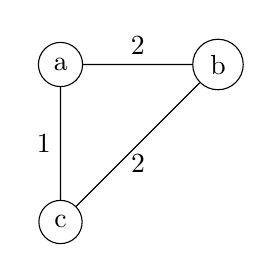
\begin{tikzpicture}
	\path 	(0, 2) node[circle, radius=2.5pt, draw] (a) {a}
			(2, 2) node[circle, radius=2.5pt, draw] (b) {b}
			(0, 0) node[circle, radius=2.5pt, draw] (c) {c};
	\draw (a) 
				-- node[above] {2} (b) 
				-- node[below] {2} (c) 
				-- node[left] {1} (a);
\end{tikzpicture}
	\label{fig:figure1}
\end{figure}
The tree containing two edges $(a, b), (b, c)$ is an MBT but is clearly
not a MST.

\subsection*{b}
\begin{proposition}
We will show that given an undirect graph $G$ with distinct edge
cost, if $T$ is $G$'s minimum spanning
tree (MST) then it is also a minimum-bottleneck tree (MBT) of $G$.	
\end{proposition}
\begin{proof}
	We will prove by contradition. That is, let $T$ be an MST of $G$,
	there must exist a spanning tree $T'$ whose maximum edge cost
	being smaller than the maximum edge cost of $T$.
	Let $e_i$ and $e'_i$ denote the edges of $T$ and $T'$ respectively.
	This means
	\[
		\max_i{e'_i} < \max_i{e_i}.
	\]

	Let the maximum edge of $T$ be $e_j$, we thus have
	\[
		\forall i, e'_i < e_j.
	\]

	Now consider the cut $(S, V\setminus S)$ that $e_j$ is the corresponding
	safe edge, there must exist an edge $e'_j$ in $T'$ that also crosses $(S, V\setminus S)$.
	We thus have
	\[
		e'_j < e_j \leq e'_j
	\]
	which is clearly a contradition.
\end{proof}
\section*{Exercise 4}
\subsection*{a}

\begin{algorithm}[H]
	\caption{Check for MST($G, T, c$)}
	Let $P=(e_1, ..., e_n)$ be the cycle computed with DFS($T \cup \{c\}$)\;
	\eIf{$c$ is the edge with largest cost in $P$}{
		\Return False \tcp*{$T$ remains the MST}
	}
	{
		\Return True \tcp*{$T$ does not remain the MST}
	}

\end{algorithm}

Complexity $O(n)$ since it is dominated by DFS algorithm.

\subsection*{b}
\begin{algorithm}[H]
	\caption{Fix MST($G, T, c$)}
	Let $P=(e_1, ..., e_n)$ be the cycle computed with DFS($T \cup \{c\}$)\;
	Let $e_m = \max_{i\in P} e_i$\;
	\Return $T \cup \{c\} \setminus \{e_m\}$ 

\end{algorithm}

Complexity $O(n)$ since it is dominated by DFS algorithm.


\begin{proposition}
	Let $T$ be the MST of $G(V, E)$, assuming we add a new edge $c$ to $G(V, E)$, the
	MST of the modified graph must be a subset of $T\cup \{c\}$.
\end{proposition}
\begin{proof}
	We will prove by contradiction. That is the MST of the modified graph contain some $e_i$ which
	does not belong to $T \cup \{c\}$. Suppose $e_i$ is the safe edge crossing some cut 
	$(S, V\setminus S)$ of the graph $G'(V, E \cup \{c\})$. Suppose $e_j$ is the safe edge
	crossing $(S, V\setminus S)$ of the graph $G(V, E)$. Clearly:
	\[
		e_i \neq e_j, e_i \neq c
	\]

	Now, let $E(S, V\setminus S)$ and $E'(S, V\setminus S)$ be the set of edges crossing
	the said cut in two graphs $G$ and $G'$ respectively. There are only two cases: 
	1) 
	$$E'(S, V\setminus S)=E(S, V\setminus S) \cup \{c\}$$ and 2) 
	$$E'(S, V\setminus S)=E(S, V\setminus S)$$
	In both case, $e_i \neq e_j, e_i \neq c$
	lead to contradition.

\end{proof}

\begin{proposition}
	Let $T$ be the MST of $G(V, E)$. Suppose we remove some edges which do not belong
	to $T$ from $G$, then $T$ is also the MST of the modified graph.
\end{proposition}
\begin{proof}
	We will prove this by showing that every safe edge of $G$ must also be a safe edge
	of the modifed graph $G'$. Clearly, let's assume $e_i$ is a safe edge of $G$ crossing a cut
	$(S, V\setminus S)$. Since we do not remove safe edge from $G$ to create $G'$, clearly
	$e_i$ also crosses the same cut in the modifed graph $G'$. This implies $e_i$ is also
	a safe edge of $G'$.
\end{proof}


\section*{Exercise 5}
\begin{algorithm}[H]
	\caption{Algorithm($G(V, E)$)}
	Initialize new set of vertices $V' = V$\;
	Initialize new set of edges $E' = \emptyset$\; 
	\For{$e_i$ in $E$}{
		add new edge $e'_i = -\log (1 - e_i)$ to $E'$
	}
	\Return Dijkstra($G'$)
\end{algorithm}

\subsubsection*{Analysis}
This algorithm complexity is basically the same as Dijkstra, which is 
$$O((n + m)\log n)$$

\subsubsection*{Proof of correctness}
We will show that if a set of edge $(e_1, e_2, ..., e_k)$ has the lowest
negated logarithmic cost then they have the least chance of at least
one edge failed.

Additionally, it is remarked that the negated logarithmic cost is always
positive. This ensures Dijkstra works correctly.

\begin{proof}
	Given some edge $(e_i,...)$, let the chance of having at least one failure
	be $R_f$ and the chance of all edge success be $R_s$, we have:
	\[
	 	R_f + R_s = 1
	 \] 
	 where $R_s = \prod_i{1-e_i}$.

	 Since $P = \{e_i,...\}$ has the lowest negated log cost, for any 
	 other path $P' = \{e_j,...\}$
	 we have the following
	 \[
	 	\begin{aligned}
	 		- \sum_{e_i \in P}{\log{(1 - e_i)}} &\leq - \sum_{e_i \in P'}{\log{(1 - e_i)}} \\
	 		\sum_{e_i \in P}{\log{(1 - e_i)}} &\geq \sum_{e_i \in P'}{\log{(1 - e_i)}} \\
	 		\prod_{e_i \in P}{(1 - e_i)} &\geq \prod_{e_i \in P'}{(1 - e_i)} \\
	 		R_s(P) & \geq R_s(P') \\
	 		R_f(P) & \leq R_f(P') \\
	 	\end{aligned}
	 \]
\end{proof}
\end{document}
